\section{Method}
\label{sec:methods}

\subsection{A mixture over tracers}
\label{sec:methods:mixture}

The host of a dark siren is unknown, so the analysis marginalises over it. Given
data $d_i$ for event $i$ and parameters $\Lambda$ containing the cosmology and
the source population, the single-event evidence is
\begin{equation}
  Z_i(\Lambda) = \int \dd\theta\; p(d_i \,|\, \theta)\,
                 p_{\rm pop}(m_1, m_2, \chi \,|\, \Lambda)\,
                 p(z, \hat{n} \,|\, \Lambda),
  \label{eq:zi}
\end{equation}
where $\theta$ collects source-frame masses, effective spin, redshift and sky
direction, and $p(z, \hat{n}|\Lambda)$ is the host prior supplied by the
catalog. When more than one tracer of the same underlying structure is
available, that prior becomes a mixture,
\begin{equation}
  p(z, \hat{n} \,|\, \Lambda) = \sum_{k=1}^{K} f_k \,
      p_k(z, \hat{n} \,|\, \Lambda), \qquad \sum_k f_k = 1,
  \label{eq:mixture}
\end{equation}
with $f_k$ the fraction of mergers hosted by tracer $k$. Throughout we take
$K=2$ with tracer~1 the galaxies and tracer~2 the AGN, so
$f_2 \equiv \fagn$ is the parameter of interest and $f_1 = 1 - \fagn$. Written
this way, \fagn\ is a mixture weight between two host priors and nothing else:
it does not enter the mass or spin distributions, and it is identified purely by
which tracer's redshift-and-sky structure the events prefer.

Each tracer's host prior is built from its pixelated catalog as a
kernel-density estimate in redshift, evaluated in the event's HEALPix pixel:
\begin{equation}
  p_k(z, \hat{n} \,|\, \Lambda) \;\propto\; g(z; \Lambda)
     \sum_{j \,\in\, k,\; \hat{n}_j = \hat{n}}
     \frac{w_j}{W_k}\,
     \frac{\mathcal{N}(z; z_j, \sigma_j)}{\zeta_j},
  \label{eq:pcat}
\end{equation}
where $z_j$ and $\sigma_j$ are a catalogued host's redshift and its
uncertainty, $w_j$ its weight, $g(z;\Lambda)$ the redshift weighting imposed by
the comoving volume element and the merger-rate evolution, and
$\zeta_j = \int \mathcal{N}(z; z_j, \sigma_j)\, g(z;\Lambda)\, \dd z$ normalises
each host's kernel against that weighting.

\subsection{Why the sky normalisation is the whole point}
\label{sec:methods:field}

The one convention in Equation~(\ref{eq:pcat}) that decides whether a
multitracer analysis has any information at all is the choice of $W_k$. We use
the \emph{survey-global} normalisation, $W_k = \sum_j w_j$ over the entire
catalog of tracer $k$, rather than the per-pixel sum. The difference is not
cosmetic. With a global normalisation the number of tracer-$k$ hosts in a pixel
survives into the likelihood, so a pixel that is rich in galaxies but contains
no AGN contributes weight to tracer~1 and none to tracer~2; with a per-pixel
normalisation every occupied pixel is renormalised to unity and the sky-density
contrast between the tracers is discarded. Since a sparse tracer's information
is precisely that most of the sky contains none of it --- in our clustered mocks
\GlassAgnEmptyPix\% of the \GlassNpix\ pixels hold no AGN at all, against
\GlassGalEmptyPix\% for the galaxies --- the global convention is the one under
which \fagn\ is identifiable. It also means an event localised in a pixel with
no catalogued AGN can only be AGN-hosted through the out-of-catalog term of
\S\ref{sec:methods:completion}, which is what couples \fagn\ to the assumed AGN
number density.

\subsection{Missing hosts}
\label{sec:methods:completion}

A flux-limited survey stops finding hosts beyond some redshift, and the
analysis has to say what is missing. The missing budget per tracer is set by a
smooth density model,
\begin{equation}
  \frac{\dd N_{{\rm miss},k}}{\dd z} =
    n_{0,k}\, \frac{\dd V_c}{\dd z}\, (1+z)^{\delta_k}
    - \frac{\dd N_{{\rm obs},k}}{\dd z},
  \label{eq:miss}
\end{equation}
and distributed isotropically over the sky, so completeness is never a free
function of redshift: it follows from the assumed density amplitude and
evolution together with the observed counts,
\begin{equation}
  C_k(z) = \frac{\dd N_{{\rm obs},k}/\dd z}
                {n_{0,k}\, (\dd V_c/\dd z)\, (1+z)^{\delta_k}}.
  \label{eq:completeness}
\end{equation}
This is the mechanism that lets a thinned survey still constrain \fagn: as
observed hosts disappear, each tracer's prior migrates from its own KDE onto its
own smooth field, and the two fields still differ by the number-density ratio
that carried the signal. It is also the mechanism that makes the answer depend
on $n_{0,k}$, which \S\ref{sec:density} is about. Setting
$n_{0,k} \rightarrow 0$ removes the missing budget and recovers the
complete-catalog estimator, which we use for the complete-catalog results.

Anchoring $n_{0,k}$ fixes the budget's amplitude but not its shape: the true
tracer density is whatever the mock's density field produced, not exactly
$(1+z)^{\delta}\,\dd V_c/\dd z$. We therefore anchor $n_{0,k}$ and $\delta_k$ at
the best fit of the model \emph{form} to the true host density rather than at
the raw mean density --- for the single-tracer mock,
$\log_{10} n_0 = \AncLogNzero$ and $\delta = \AncDelta$, against a raw mean
density of $\AncNaiveLogNzero$ --- and quote the residual of that fit as the
level below which an apparent completeness bias is not attributable to
completeness. That residual is \AncResidFit\% rms over the fit range and
\AncResidHorizon\% within the detection horizon, the latter dominated by the
shot noise of the \AncNHostsInHorizon\ hosts that lie there. For the two-tracer
mock the corresponding anchors are
$(\log_{10} n_0, \delta) = (\AnchorGalLogNzero, \AnchorGalDelta)$ for the
galaxies and $(\AnchorAgnLogNzero, \AnchorAgnDelta)$ for the AGN, with shape
residuals of \AnchorGalResidHorizon\% and \AnchorAgnResidHorizon\% inside the
horizon.

\subsection{Selection}
\label{sec:methods:selection}

With detection accounted for, the likelihood over $\Nobs$ detected events is
\begin{equation}
  \ln \mathcal{L}(\Lambda) = \sum_{i=1}^{\Nobs} \ln Z_i(\Lambda)
      - \Nobs \ln \mu(\Lambda),
  \label{eq:like}
\end{equation}
with $\mu(\Lambda) = \int \dd\theta\, P_{\rm det}(\theta)\, p(\theta|\Lambda)$
the detectable fraction \citep{MandelFarrGair2019}. We estimate $\mu$ by
importance sampling a campaign of injections recorded in the cosmology-free
observables $(m_1^{\rm det}, q, d_L)$ with their proposal density, and require
the estimator's effective sample size to satisfy $\Neff > 5\,\Nobs$ for the
estimate to be usable \citep{Farr2019, Vitale2022}. Grid cells that fail
that criterion are inadmissible and are shown as such in the figures; where
they occur we report how much posterior mass lies next to them, because a
posterior whose peak sits against an inadmissible edge is a statement about the
selection estimate rather than about the data.

\subsection{A sparse tracer needs its own injections}
\label{sec:methods:targeted}

The selection integral in Equation~(\ref{eq:like}) is conditioned on the host
catalog through Equation~(\ref{eq:pcat}), so an injection carries weight only if
its redshift lands within a few $\sigma_j$ of an actual catalogued host
\emph{in its own pixel}. As \fagn\ rises, $\mu$ leans on the sparse tracer, and
injections drawn from the source population essentially never land on it. This
is not a nuisance: it changes the answer. We therefore draw injections from a
three-branch mixture --- \InjWpop\ from the source population, \InjWuni\
uniform, and \InjWtgt\ placed at catalogued AGN --- and store, for every
injection, the exact mixture density at its own coordinates. Two properties
make the construction safe. The targeted branch reads the \emph{pixelated
survey file}, which is the object the likelihood conditions on and whose stored
redshifts and widths are the kernel centres and widths of
Equation~(\ref{eq:pcat}), so proposal and target cannot drift apart through a
pixelisation or kernel-width mismatch; and the stored densities were recomputed
by an independent code path, agreeing to a maximum relative error of
$\InjPdrawErr$. From \InjNdraw\ million proposals, \InjNdet\ are detected, of
which \InjOnAgnSupport\% fall on AGN catalog support, against \InjOnAgnPop\%
for population draws and \InjOnAgnUni\% for uniform ones, while the detected
fraction $\InjFracDet$ stays within a few per cent of the untargeted campaign's.

Across a completeness ladder the support the likelihood conditions on shrinks
with the survey, so one injection set per rung is generated against that rung's
own catalogs. Holding the branch \emph{weights} fixed along the ladder is the
wrong invariant: a flux limit leaves only bright, nearby hosts, so the targeted
branch's detection efficiency climbs steeply and, at fixed weights, the campaign
fills with targeted rows carrying negligible weight while starving the
population branch --- the one branch that covers the out-of-catalog term, which
is exactly the term that grows as the survey empties. We hold the fraction of
\emph{detected} rows contributed by each branch fixed instead, solving for the
weights from a per-rung pilot run.

\subsection{The catalog's redshift resolution is not free}
\label{sec:methods:kde}

The kernel widths $\sigma_j$ in Equation~(\ref{eq:pcat}) have to sit inside a
window bounded on both sides, and both bounds are measured.

The lower bound is computational, and it is a genuine design tension rather
than a numerical detail. Narrow kernels --- spectroscopic redshift errors,
say --- make each tracer's prior a set of thin shells in redshift, which
sharpens the dark-siren information but shrinks the support the selection
integral has to cover, driving $\Neff$ down and the per-event Monte Carlo
variance up. On the matched single-tracer mock, pixelating the same catalog
with its survey-style spectroscopic widths (median $\KwDzSpecMed$) instead of
our adopted $\dd z = \GlassDzScale$ cuts the selection integral's effective
sample size at the truth from \KwNeffAdopt\ to \KwNeffSpec\ --- below the
$5\,\Nobs = \KwFloor$ floor, so the scan is not even admissible --- while
quadrupling the summed per-event Monte Carlo variance (\KwPeVarAdopt\ to
\KwPeVarSpec). Widening the kernels buys that resolution back at the direct
cost of the signal, because the catalog's redshift precision \emph{is} the
dark-siren information. At the adopted width the two-tracer complete rung has
$\Neff = \IncCompleteNeff \times 10^3$ against a floor of \IncGuardFloor, with
a summed per-event log-likelihood variance of \IncPeVarComplete.

The upper bound is a threshold in the inference itself, not a slow
degradation, and it is set by the scale the kernels must never approach: the
parameter estimates' own redshift resolution, $\sigma_z^{\rm PE} \simeq
\sigma_{d_L}\, d_L\, (\dd d_L/\dd z)^{-1}$, which is \SkdePeZWidth\ at the
median event of the matched mock. Broadening the catalog kernels at fixed data
leaves the recovered expansion rate flat within \SkdeFlatSpread~\kmsmpc\ up to
an effective kernel width of \SkdeEffTwenty\ --- still under the PE resolution
--- and then fails catastrophically: \SkdeThirtyOff~\kmsmpc\ at
\SkdeEffThirty, \SkdeFortyOff\ at \SkdeEffForty, \SkdeSeventyOff\ at
\SkdeEffSeventy, reproduced on a second realisation (\SkdeSFortyOff\ at
\SkdeEffForty; Figure~\ref{fig:kernelthresh}). Once the host prior is as broad as the
measurement, the likelihood's redshift information comes from the prior's
overlap with the moving posterior rather than from the hosts, and the
distance scale runs away. The design rule for a real survey follows directly,
and it is a statement about photometric redshifts: catalog redshift kernels
--- including any photo-$z$ scatter they encode --- must stay well below the
distance posteriors' implied redshift width, or the catalog stops being a
redshift prior and becomes a redshift bias.

\begin{figure}
\centering
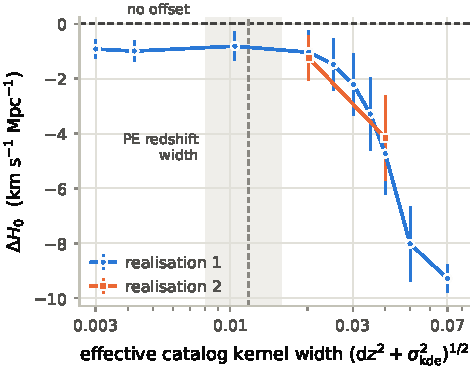
\includegraphics[width=\columnwidth]{figures/fig_kernel_threshold.pdf}
\caption{The catalog kernel width is a threshold lever. Recovered
expansion-rate offset against the effective kernel width
$(\dd z^2 + \sigma_{\rm kde}^2)^{1/2}$ when the catalog kernels are broadened
at fixed data, for two independent realisations of the matched single-tracer
mock. The band marks the 16--84\% range of the per-event PE redshift width
$\sigma_{d_L}\, d_L\, (\dd d_L/\dd z)^{-1}$; the offset is flat until the
kernels approach it, then runs away.
\label{fig:kernelthresh}}
\end{figure}

\subsection{Mocks}
\label{sec:methods:mocks}

Two families of mocks are used, and they answer different questions.

\emph{Clustered two-tracer mocks.} The flagship $K=2$ measurements use
lognormal density fields generated with \textsc{glass}
\citep{Tessore2023}, sampled into two biased tracers: \GlassNgal\
galaxies with linear bias \GlassBiasGal\ and \GlassNagn\ AGN with linear bias
\GlassBiasAgn, out to $z = \GlassZmax$, on a HEALPix grid with
$N_{\rm side} = \GlassNside$. The resulting comoving number densities are
$\log_{10} n_0 = \GlassGalLogNzero$ and \GlassAgnLogNzero, a ratio of
\GlassDensityRatio, and \GlassAgnEmptyPix\% of pixels contain no AGN. Events
are \GlassNobs\ mergers whose hosts are drawn from the two host lists in the
planted proportion, with source redshifts restricted to $z \le \GlassZtrunc$;
masses and spins are drawn from a power-law-plus-peak population at fiducial
values, and each event carries \GlassNsamp\ posterior samples built by exact
inverse-transform sampling of the flat-prior posterior given a noisy
observation, with a fractional distance uncertainty of \GlassDlUnc. These mocks
carry the clustering-bias contrast, which is the physical channel the paper is
about; their detection rule is a hard cut on true source redshift, which is the
one place where their generative process is not the inference's model.
Section~\ref{sec:selection:tilt} measures exactly what that inconsistency does
to the recovered distance scale, and \S\ref{sec:disc:limits} states what the
clustered mocks can and cannot be used for because of it.

\emph{Matched mocks.} To measure the error budget of the inference itself we
need mocks whose generative process \emph{is} the assumed model, ingredient by
ingredient. These are generated end to end by the inference code's own mock
generator: detection is a noisy network signal-to-noise threshold on an
observable, hosts are accepted with the same redshift weighting the likelihood
assumes, and masses, spins and posterior samples come from the same samplers the
likelihood uses. That standard is not automatic even for a generator built for
it: \S\ref{sec:budget} shows the generator as first shipped violated it in
three measured respects --- posterior samples centred on the truth, a
detection decision taken on latent data, and a sky-localisation width derived
from latent parameters --- each identified and repaired there. Except where a
comparison against the original generator is itself the point, every
matched-mock result in this paper comes from the repaired generator, in which
every quantity the likelihood conditions on is a function of the observed
data. The single-tracer version has \CloNhosts\ hosts out to
$z = \CloZmax$ --- far beyond the events, so the catalog's redshift boundary
cannot shape the prior where the data live --- pixelated complete at
$N_{\rm side} = \CloNside$ with \CloEmptyPix\% empty pixels, \CloNobs\ events
with \CloNsamp\ posterior samples each and a fractional distance uncertainty of
\CloSeedSigmaDl, and a selection campaign of \CloInjNdraw\ million proposals of
which \CloInjNdet\ are detected. The two-tracer version has \DeepNgalHosts\
galaxies and a nested subset of \DeepNagnHosts\ AGN
($\log_{10} n_0 = \DeepGalLogNzero$ and \DeepAgnLogNzero, with
\DeepAgnEmpty\% of AGN pixels empty), \DeepNgalEvents\ galaxy-hosted plus
\DeepNagnEvents\ AGN-hosted events at a planted $\fagn = \DeepFTruth$, and
$N_{\rm side} = \DeepNside$. Their scope limit is stated up front: the
generator's catalogs are unclustered, so in these mocks \fagn\ is identified by
the number-density contrast alone with none of the bias contrast the clustered
mocks carry. The two families are complementary, not redundant.

\emph{The completeness ladder.} Incompleteness is imposed as an isotropic
apparent-magnitude limit on the complete catalog --- no footprint, no hard
redshift cut --- so that completeness is a \emph{consequence} of survey depth
and has the declining shape a flux-limited survey actually has. The events are
untouched: incompleteness is an observational effect, so the mergers are exactly
the ones that happened, and only the catalogs the inference sees are thinned. In
the two-tracer ladder the AGN are a nested subset of the galaxies and inherit
their host galaxy's apparent magnitude, so one flux limit thins both tracers
with the same $C(z)$ and the ladder stays a single-axis experiment.

\subsection{Inference}
\label{sec:methods:inference}

We evaluate the likelihood of Equation~(\ref{eq:like}) directly on grids rather
than sampling it, which is affordable because at most three parameters are free
at a time and which removes any question of sampler convergence from the
comparisons. Flat priors are used throughout, and we quote medians with
equal-tailed 68\% and 90\% intervals; where the truth lies on a prior boundary
we say so and quote the one-sided limit instead. $\Omega_{m,0}$ is pinned at
\OmZeroTruth\ and the mass and spin population is held at the mock's truth, so
the mass distribution is informative but not free; the fiducial expansion rate
is $\Hz = \HzeroTruth$~\kmsmpc. Unless stated otherwise the sampled parameters
are \Hz\ and \fagn, with the tracer densities anchored as in
\S\ref{sec:methods:completion}; \S\ref{sec:density} adds \lognzagn.
